\documentclass[UTF8,a4paper,12pt]{ctexart}

\usepackage[margin=2.35cm]{geometry}
\usepackage{graphicx}
\usepackage{booktabs}
\usepackage{amsmath}
\usepackage{amssymb}
\usepackage{xcolor}
\usepackage{hyperref}
\usepackage{caption}
\usepackage{subcaption}
\usepackage{enumitem}
\usepackage{fancyhdr}
\usepackage{titlesec}
\usepackage{float}

\hypersetup{
  colorlinks=true,
  linkcolor=blue!55!black,
  citecolor=blue!55!black,
  urlcolor=blue!55!black
}

\graphicspath{{../output/figures/}}

\setlist[itemize]{leftmargin=2em,itemsep=0.2em,topsep=0.25em}
\setlist[enumerate]{leftmargin=2.2em,itemsep=0.2em,topsep=0.25em}
\captionsetup{font=small,labelfont=bf}

\pagestyle{fancy}
\setlength{\headheight}{14.5pt}
\fancyhf{}
\lhead{电控强耦合激子超表面光束偏转}
\rhead{\thepage}
\renewcommand{\headrulewidth}{0.4pt}

\titleformat{\section}{\Large\bfseries}{\thesection}{0.7em}{}
\titleformat{\subsection}{\large\bfseries}{\thesubsection}{0.7em}{}

\newcommand{\vg}{V_{\mathrm{g}}}
\newcommand{\gammax}{\gamma_{\mathrm{x}}}
\newcommand{\imagunit}{\mathrm{i}}

\title{\textbf{基于电控强耦合 MoSe2/WS2 激子超表面的可编程光束偏转实验设计}\\
\large Electrically Programmable Beam Steering in a Strong-Coupling Hybrid-2D Excitonic Metasurface}
\author{OPCTICAL-CHANGE / test1}
\date{2026年6月}

\begin{document}

\maketitle

\begin{abstract}
本报告整理了一个基于二维过渡金属硫族化合物（TMD）激子超表面的创新实验设计。主线不是复现已有文献图，而是把 active van der Waals MoSe2 excitonic beam steering 的裸激子相控阵，升级为 gate-tunable exciton-polariton phased array。方案利用电压调节载流子密度和 exciton linewidth，使 hybrid-2D metasurface 的 complex reflection coefficient 发生可编程变化，再通过反向设计的相位梯度实现 reflected beam steering。Python 部分采用 coupled-oscillator model、inverse phase lookup 和 one-dimensional array factor，生成五组确定性模拟图，用于验证从 gate voltage 到 far-field peak 的机制链条。所有模拟结果都是设计预测，不是实验测量数据。
\end{abstract}

\section{项目目标与核心创新}

主论文 A 已经说明，monolayer MoSe2 excitonic metasurface 能够调控反射光的 amplitude、phase 和 wavefront，并实现约 $-30^\circ$ 到 $+30^\circ$ 的 reflected beam steering。这个结果证明二维 TMD 激子可以作为主动光场调控平台，但 bare-exciton phase tuning 往往会伴随 amplitude loss，导致相位控制和偏转效率之间存在张力。

本项目的核心创新是：把主论文 A 的 bare-exciton phased array 升级为 electrically controlled strong-coupling exciton-polariton phased array。换句话说，控制对象不再只是裸激子共振附近的反射相位，而是每个 metapixel 的复反射系数
\begin{equation}
  r(\vg)=|r(\vg)|\exp[\imagunit \phi(\vg)].
\end{equation}
当 gate voltage 改变 exciton non-radiative decay / linewidth 后，强耦合状态和反射相位随之改变。多个 metapixel 组合成相位梯度，即可把反射光主瓣推到设定角度。

本方案同时保留一个支撑分析：amplitude--phase trade-off 是强耦合反射调制中必须正视的设计问题。报告中的第五张图不再使用手工 one-layer/two-layer 补偿曲线，而是回到同一 coupled-oscillator model，比较不同 photon energy 工作点下 phase span 与 amplitude CV 的取舍。

\section{文献基础与可迁移方法}

\subsection{主论文 A：active vdW excitonic beam steering}

Melissa Li、Claudio U. Hail、Souvik Biswas 和 Harry A. Atwater 在 \emph{Nano Letters} 2023 年发表的工作 ``Excitonic Beam Steering in an Active van der Waals Metasurface'' 展示了 monolayer MoSe2 active vdW metasurface 的动态反射波前控制。该系统基于 MoSe2 excitonic resonances 调节 reflection amplitude 和 phase，并在 excitonic resonances 附近实现 reflected beam steering。

本项目把这篇论文作为实验平台和问题来源：平台已经具备 beam steering 能力，短板是 bare exciton 调相位时 amplitude loss 难以完全避免。

\subsection{方法 B1：electrically tunable strong coupling}

Tom Hoekstra 和 Jorik van de Groep 的 ``Electrically tunable strong coupling in a hybrid-2D excitonic metasurface for optical modulation'' 已作为 \emph{Light: Science \& Applications} 2026 年论文发表。该工作说明，gate-tunable 2D semiconductor heterostructure 与 non-local dielectric metasurface 可以在室温下实现 electrically tunable exciton-photon strong coupling。其关键机制是 gate-induced carrier density 改变 exciton non-radiative decay rate，从而使系统经历 continuous strong-to-weak coupling transition。文献中的 9.9 dB reflectance modulation 属于该 optical modulation device 的结果，本项目只把它作为机制依据，不声称自己的 beam-steering 设计已经实现这个数值。

\subsection{方法 B2：complex amplitude control}

Hoekstra、Brongersma 和 van de Groep 的 \emph{Nano Letters} 2026 年工作 ``Hybrid-2D Excitonic Metasurfaces for Complex Amplitude Modulation'' 提供了 amplitude--phase control 的支撑思路。该工作数值展示了 hybrid-2D excitonic metasurface 的 independent amplitude and phase control，并指出引入第二层可调 monolayer 可以扩展到完整 $0$--$2\pi$ phase range。本报告只把它作为设计背景；第五张图改为由当前 coupled-oscillator model 直接导出的工作能量取舍图。

\section{物理机制与实验设计}

项目的物理链条为
\begin{equation}
  \vg \rightarrow \gammax(\vg) \rightarrow r(\vg)=|r|\exp(\imagunit\phi)
  \rightarrow \phi_j=k_0x_j\sin\theta_0 \rightarrow I(\theta).
\end{equation}
其中 $\vg$ 是 gate voltage，$\gammax$ 是 gate-dependent exciton linewidth，$r(\vg)$ 是 design energy 下的 metapixel complex reflection coefficient，$x_j$ 是第 $j$ 个 metapixel 的位置，$\theta_0$ 是目标偏转角。

样品概念可以采用 reflection geometry：
\begin{itemize}
  \item non-local dielectric metasurface；
  \item hBN / monolayer MoSe2 or WS2 / hBN；
  \item transparent top gate 或 patterned local gates；
  \item bottom gate / substrate。
\end{itemize}
支撑拓展可继续考虑 hBN-separated WS2 / MoSe2 two-layer TMD stack，但当前图件只展示 coupled-oscillator model 内部的 phase--amplitude trade-off，不把双层补偿当作已完成仿真。

实验测量流程为：
\begin{enumerate}
  \item 用 tunable laser 扫 photon energy，并同步扫 gate voltage，测得 $R(E,\vg)$。
  \item 用 coupled-oscillator model 拟合或解释谱线，提取 design energy 下的 $r(\vg)$。
  \item 选择目标角，例如 $0^\circ$、$10^\circ$、$20^\circ$。
  \item 根据 $\phi_j=k_0x_j\sin\theta_0$ 生成目标相位梯度。
  \item 从 $\phi(\vg)$ 反查每个 metapixel 所需 gate voltage。
  \item 用 Fourier-plane imaging 测 reflected far field，检查主瓣是否移动到目标角。
\end{enumerate}

\section{Python 模型}

Python 模型是设计预测模型，不是 full-wave simulation，也不是实验数据拟合。默认参数包括：design energy $1.695\,\mathrm{eV}$、wavelength $710\,\mathrm{nm}$、metapixel count $96$、metapixel spacing $0.32\,\mu\mathrm{m}$、目标角 $0^\circ/10^\circ/20^\circ$。

单元响应使用 coupled-oscillator expression：
\begin{equation}
  r(E,\vg)=r_{\mathrm{bg}}-\frac{A}
  {E_{\mathrm{c}}-E-\imagunit\kappa/2-\frac{g^2}{E_{\mathrm{x}}-E-\imagunit\gammax(\vg)/2}},
\end{equation}
其中 $E_{\mathrm{c}}$ 和 $E_{\mathrm{x}}$ 分别是 cavity mode 和 exciton energy，$g$ 是 coupling strength，$\kappa$ 是 cavity loss，$A$ 是 radiative strength，$r_{\mathrm{bg}}$ 是 background reflection。

远场使用一维 array factor：
\begin{equation}
  I(\theta)=\left|\sum_{j=1}^{N} a_j
  \exp\{\imagunit[\phi_j-k_0x_j\sin(\theta)]\}\right|^2,
\end{equation}
其中 $a_j$ 和 $\phi_j$ 来自 gate-selected complex reflection coefficient。该模型足以检查机制链：电压是否能调单元、单元是否能形成相位梯度、相位梯度是否能在 far field 中产生目标主瓣。

\section{模拟结果}

\begin{figure}[H]
  \centering
  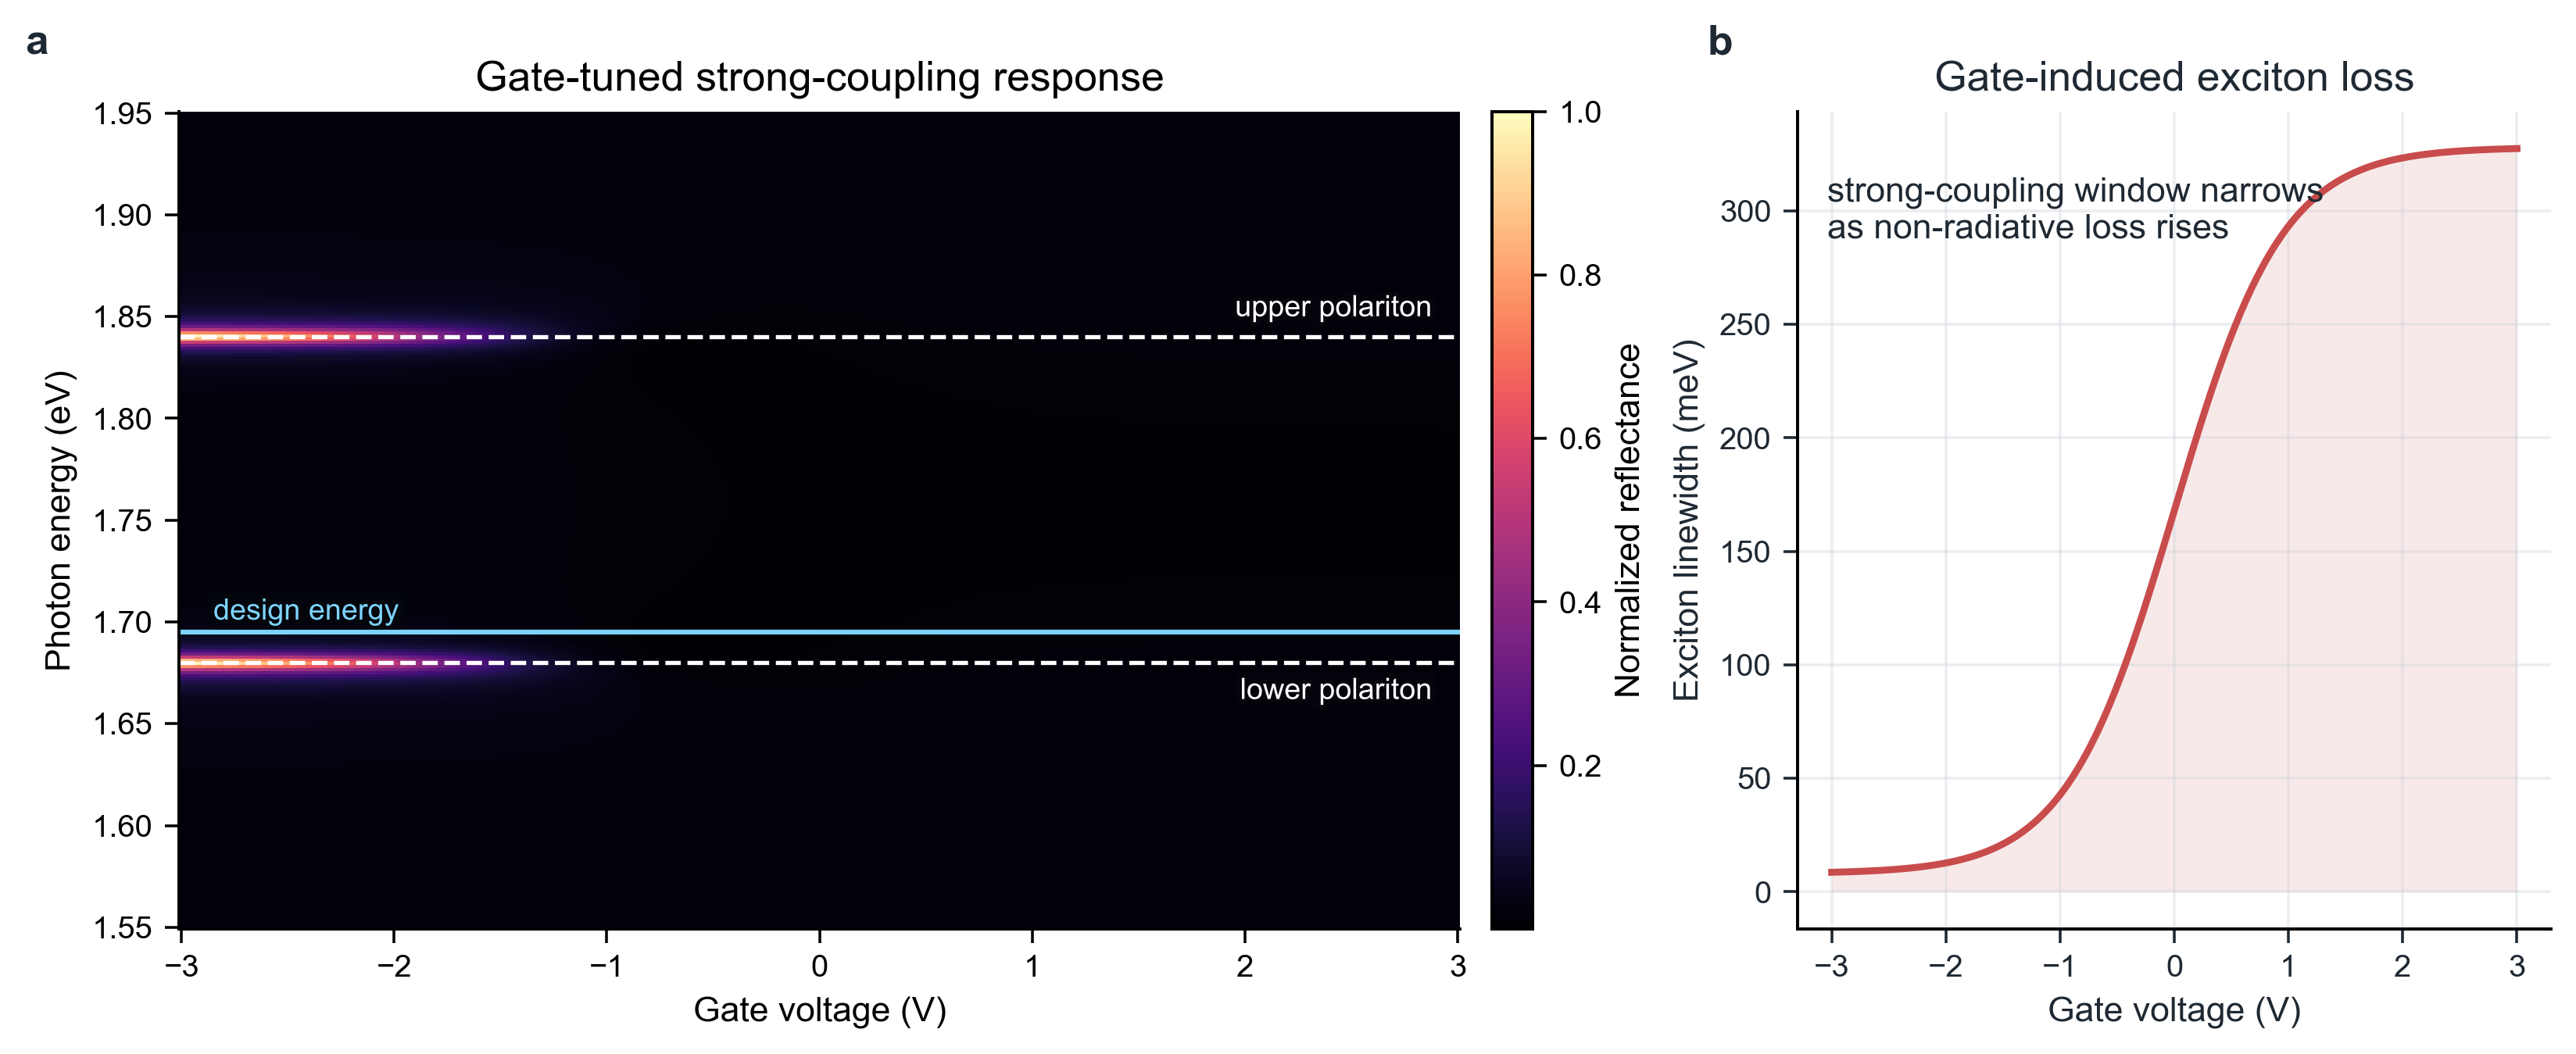
\includegraphics[width=\linewidth]{figure_1_strong_coupling_gate_tuning.png}
  \caption{Gate-tuned coupled-oscillator reflection map。左图展示 photon energy 与 gate voltage 维度上的 normalized reflectance；右图展示 gate-induced exciton linewidth broadening。该图说明 gate voltage 可以把 strong-coupling spectral feature 推向高损耗弱耦合状态。}
  \label{fig:strong-coupling}
\end{figure}

\begin{figure}[H]
  \centering
  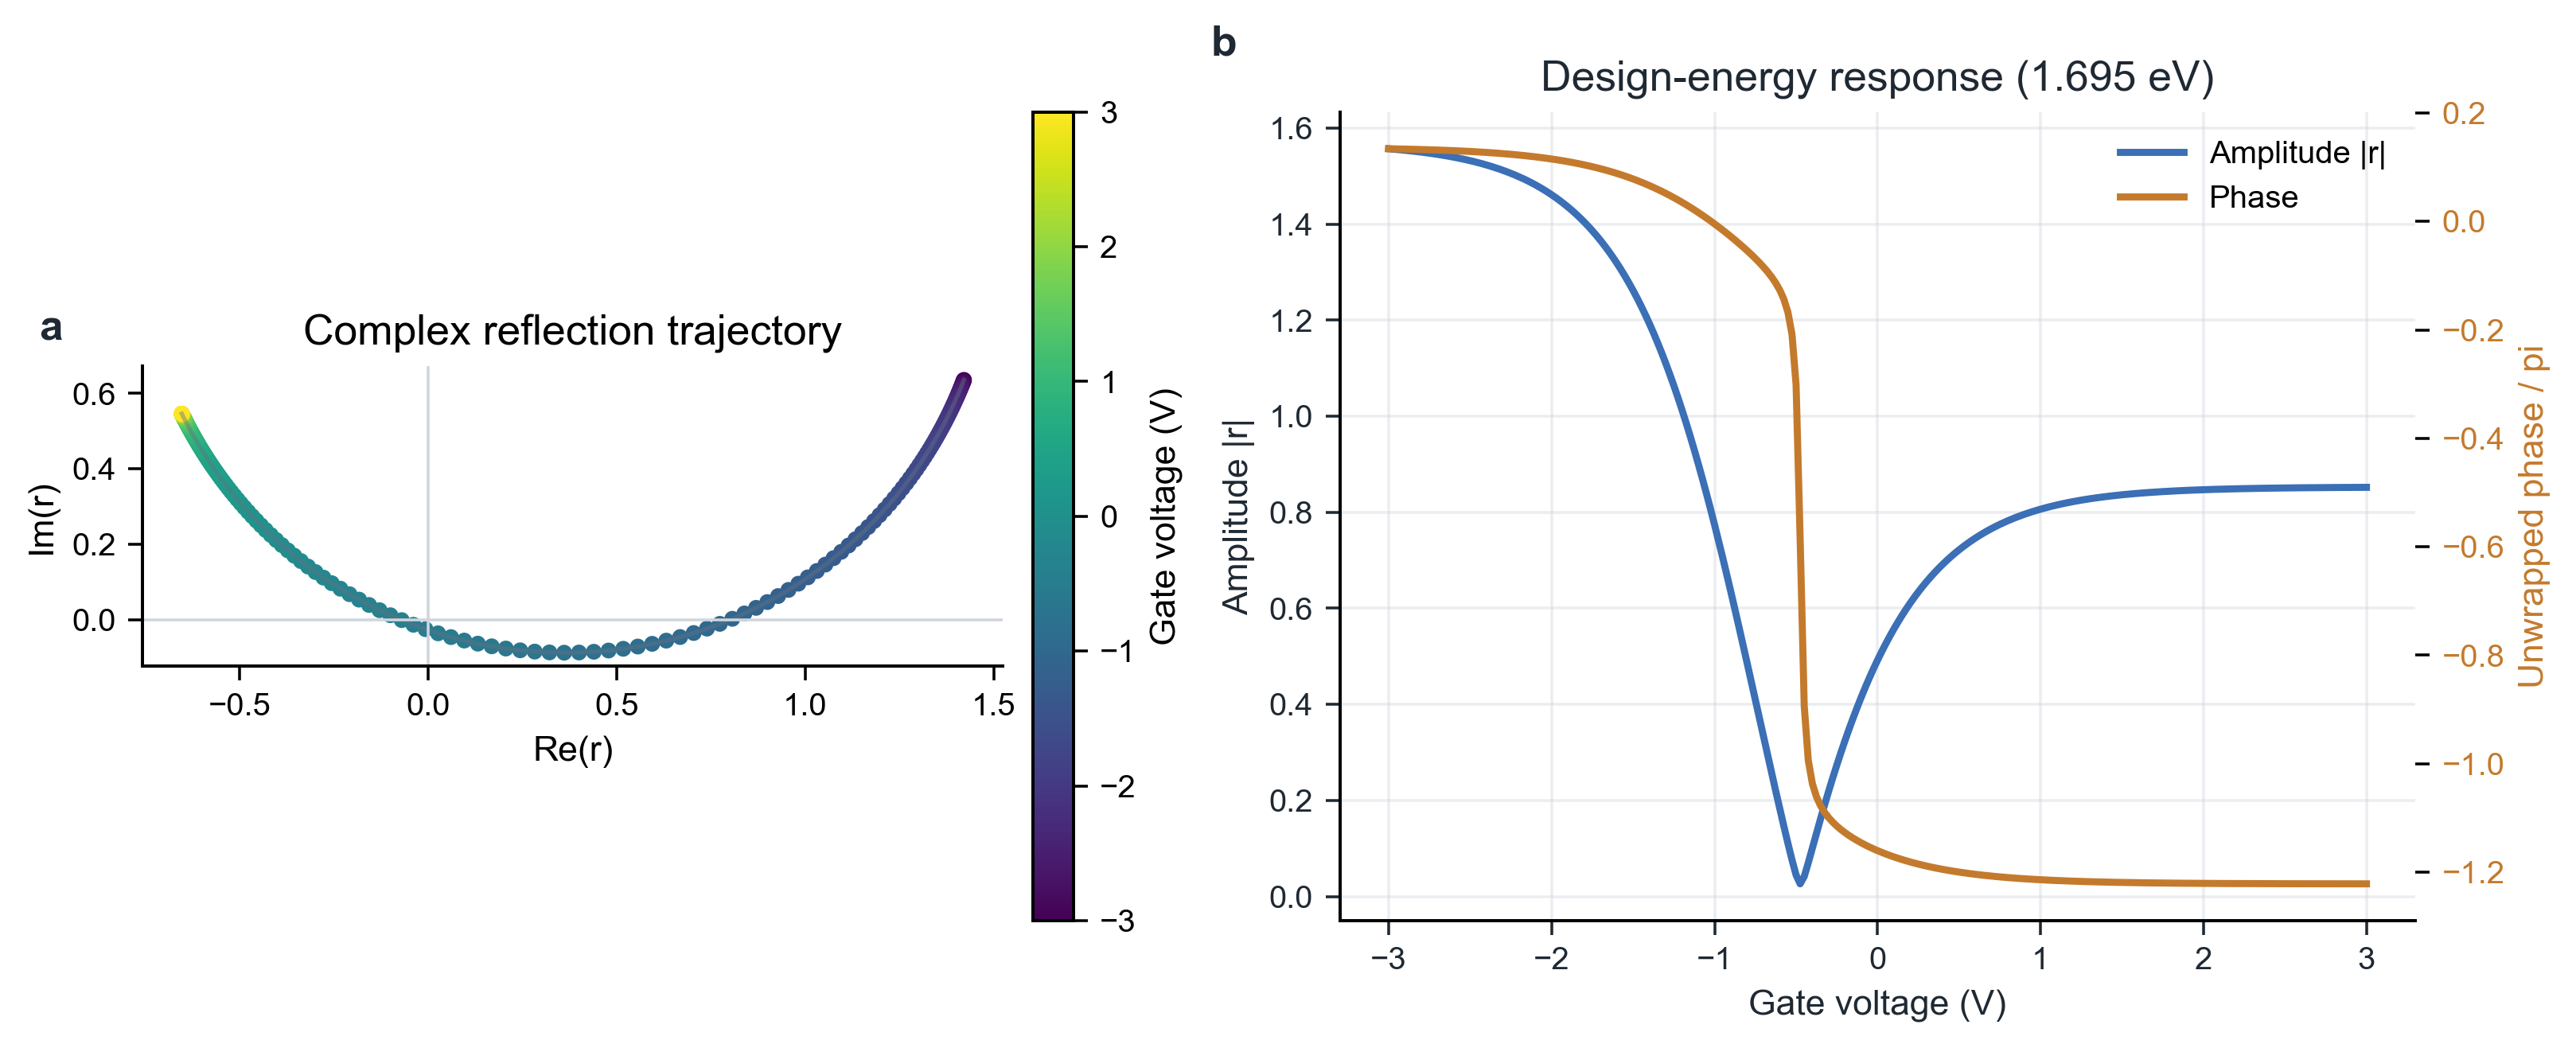
\includegraphics[width=\linewidth]{figure_2_complex_reflection_coefficient.png}
  \caption{Design energy 下的 complex reflection coefficient。左图为 $r(\vg)$ 的 complex-plane trajectory，右图为 amplitude 和 unwrapped phase 随 gate voltage 的变化。该图是反向设计的单元响应基础。}
  \label{fig:complex-reflection}
\end{figure}

\begin{figure}[H]
  \centering
  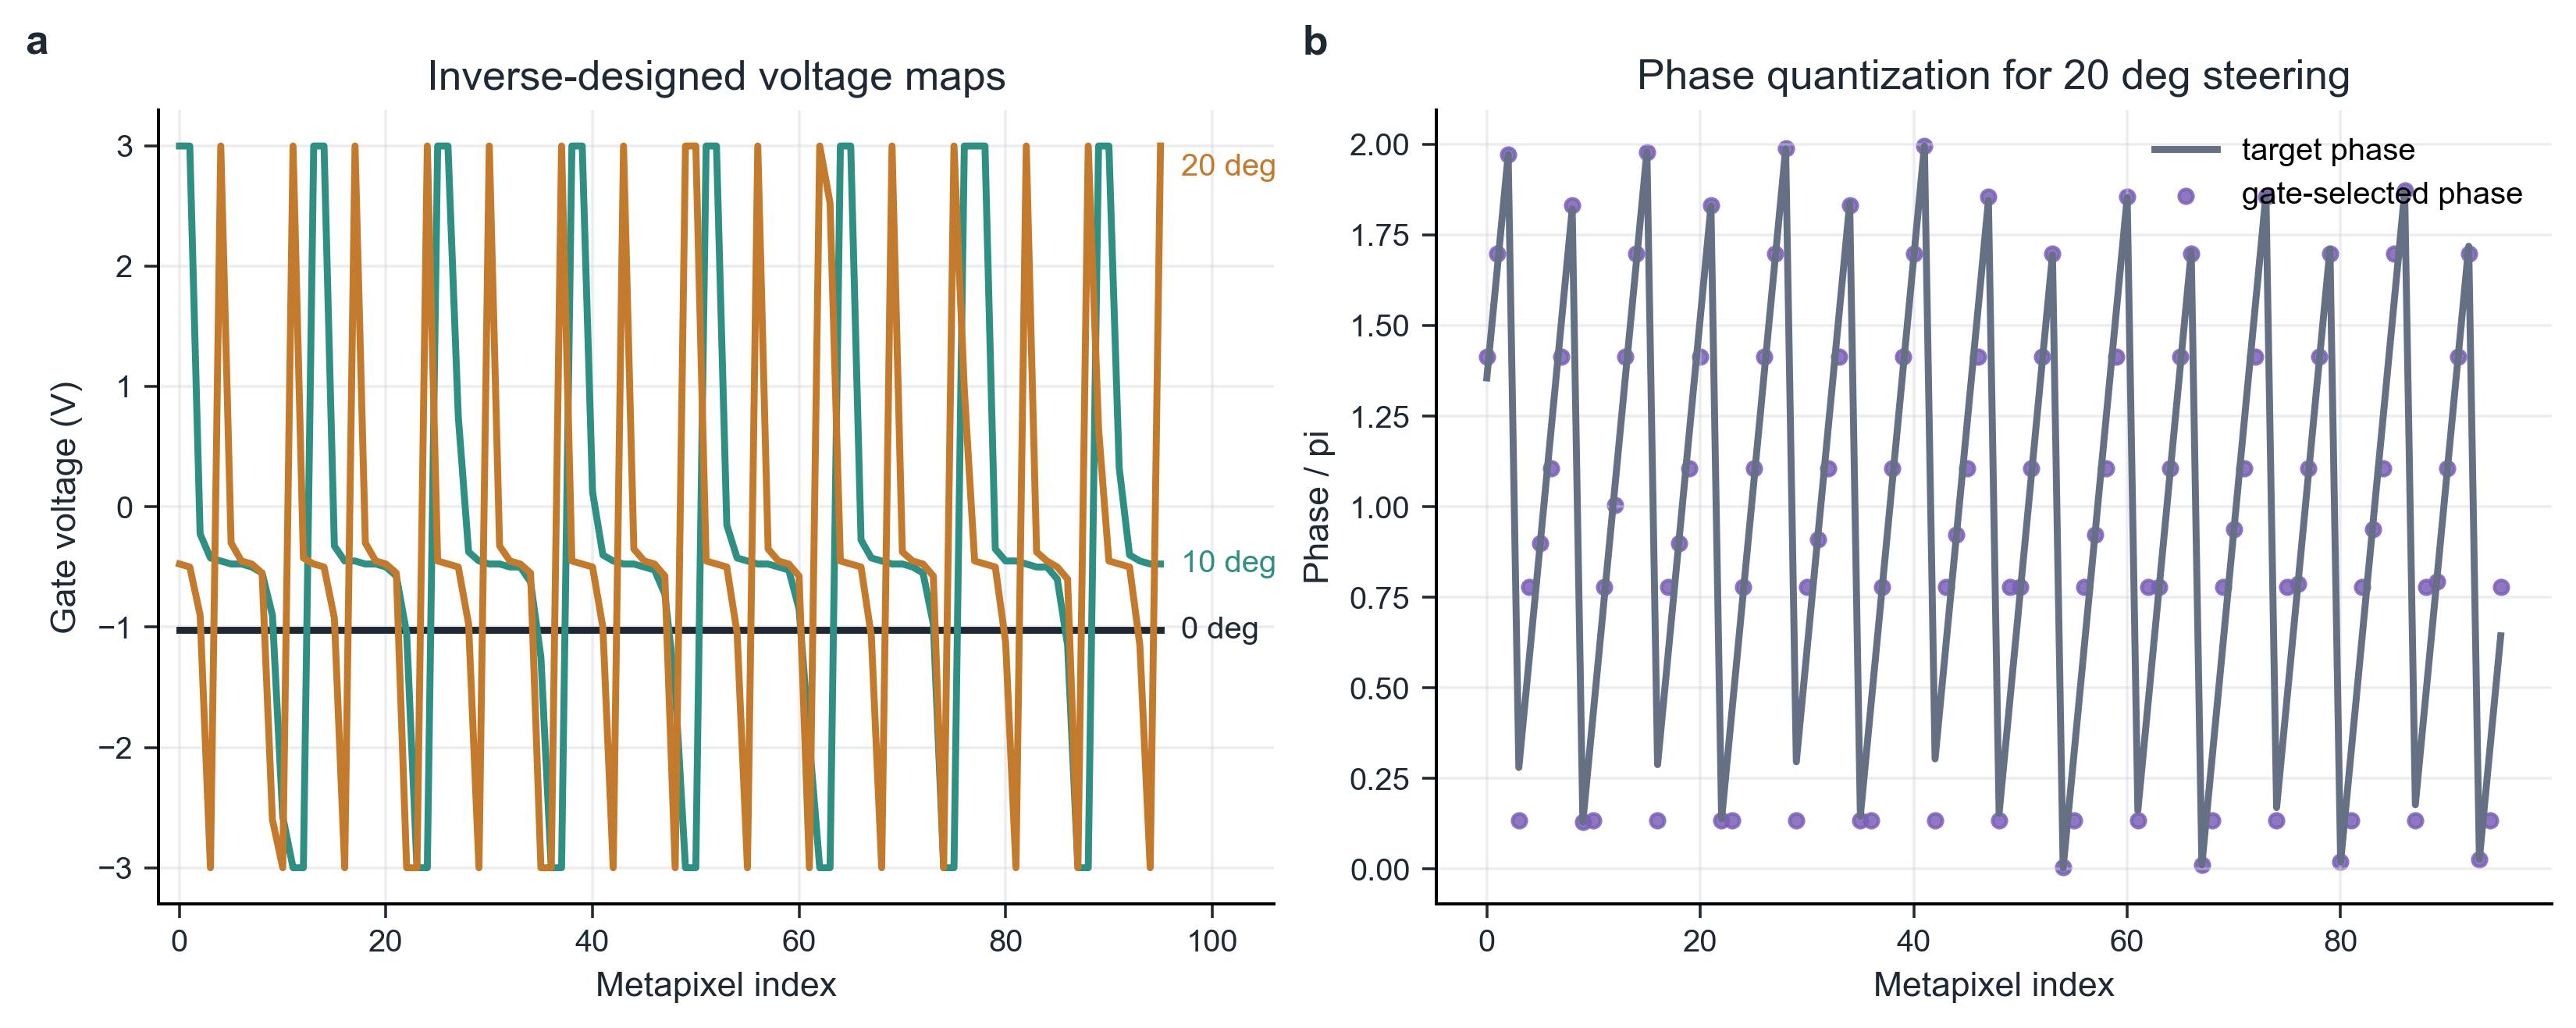
\includegraphics[width=\linewidth]{figure_3_inverse_gate_profile.png}
  \caption{Inverse-designed gate voltage profile。给定 $0^\circ$、$10^\circ$、$20^\circ$ 目标角后，模型先生成目标相位梯度，再从 $r(\vg)$ 中反查每个 metapixel 的 gate voltage。右图展示 $20^\circ$ 情况下 target phase 与 gate-selected phase 的匹配。}
  \label{fig:inverse-gate}
\end{figure}

\begin{figure}[H]
  \centering
  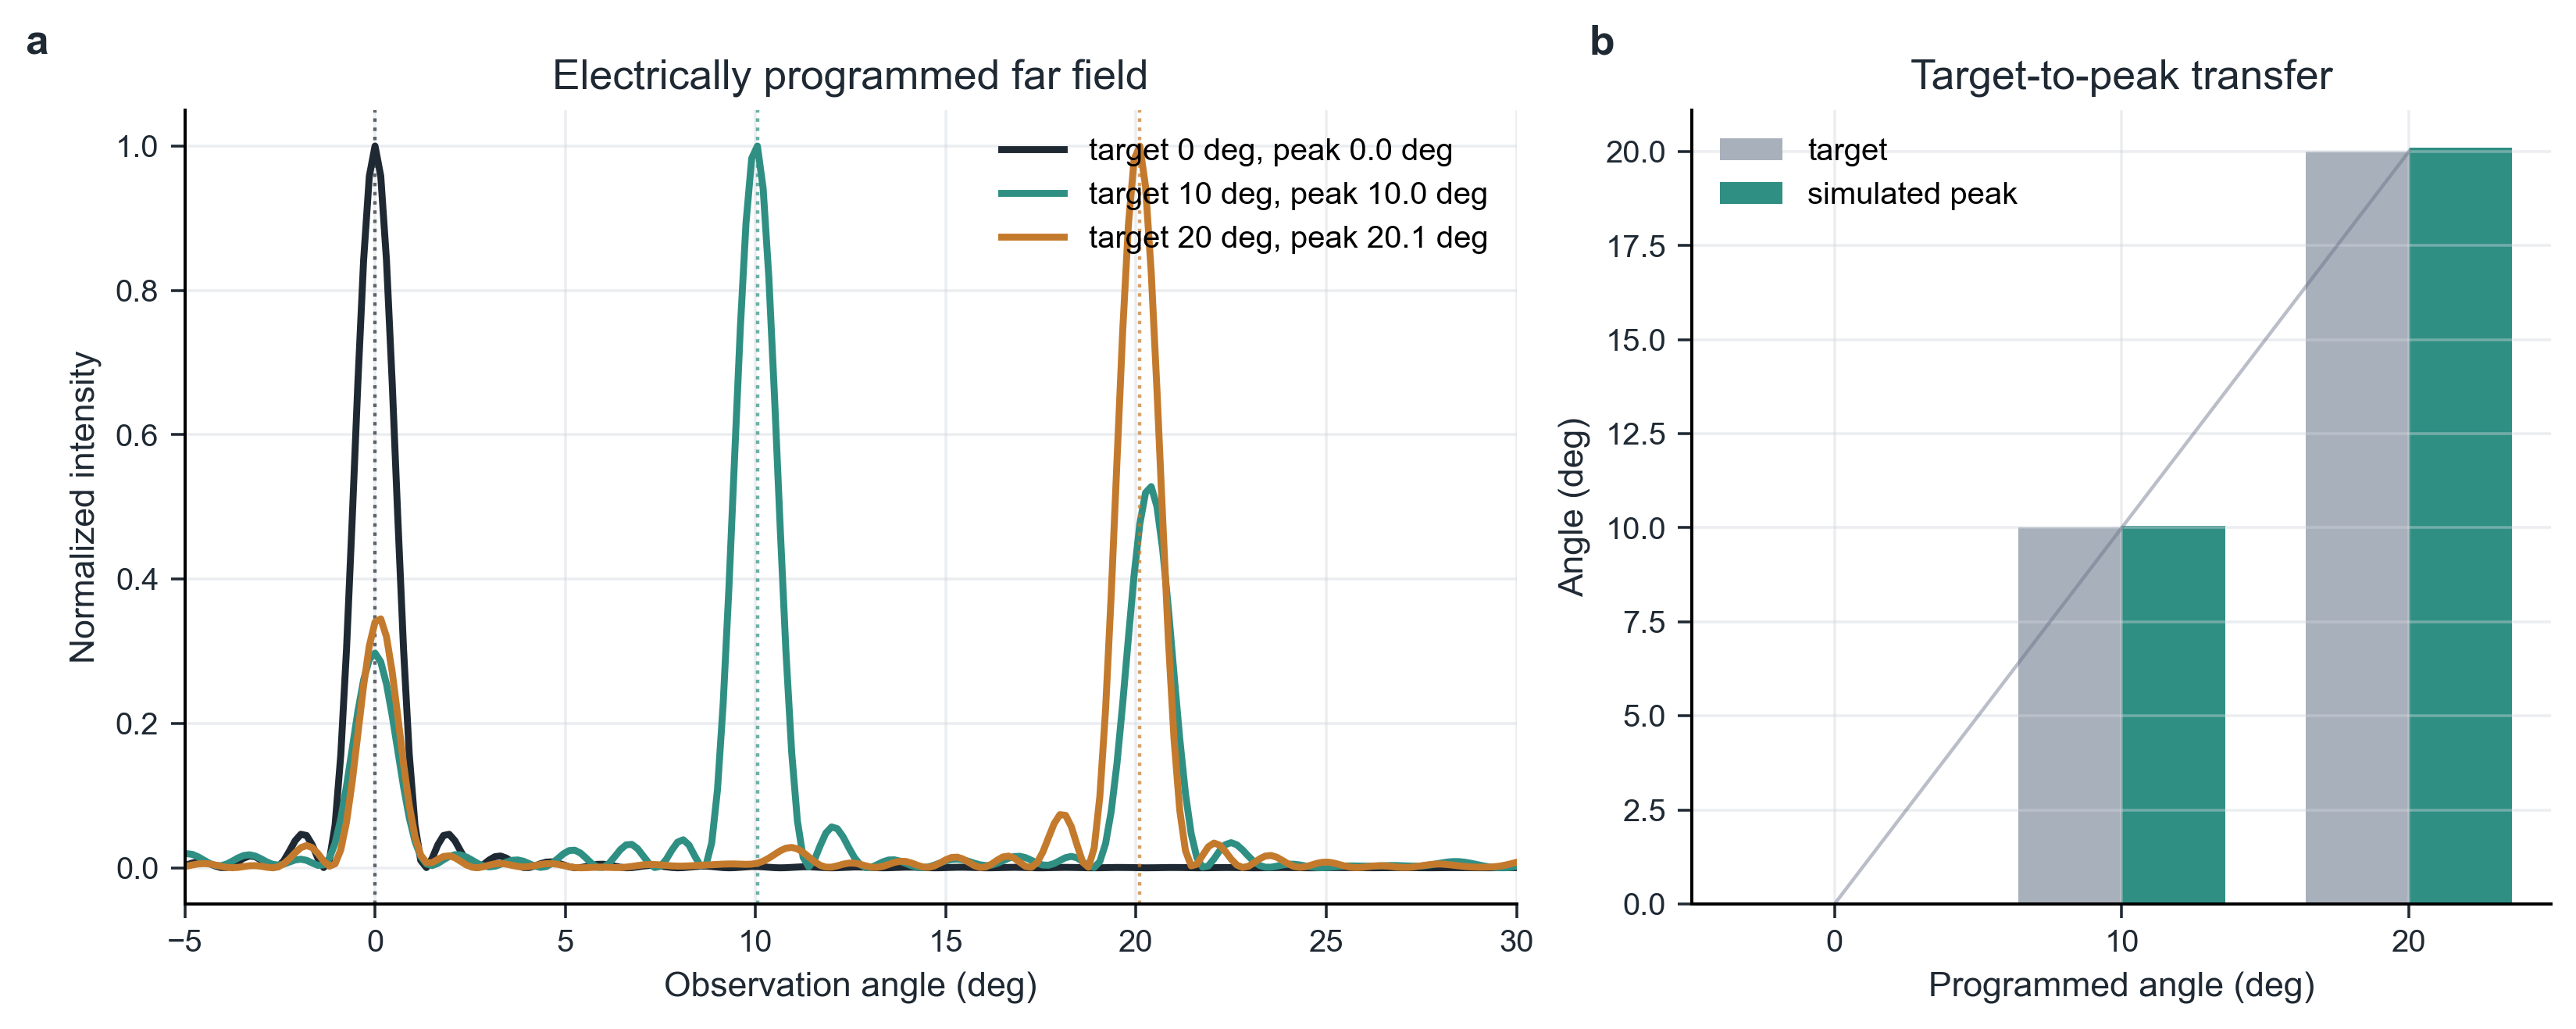
\includegraphics[width=\linewidth]{figure_4_programmable_beam_steering.png}
  \caption{Electrically programmable far-field beam steering。阵列因子结果显示，目标 $0^\circ$、$10^\circ$、$20^\circ$ 分别对应约 $0.0^\circ$、$10.0^\circ$、$20.1^\circ$ 的 far-field peak。}
  \label{fig:beam-steering}
\end{figure}

\begin{figure}[H]
  \centering
  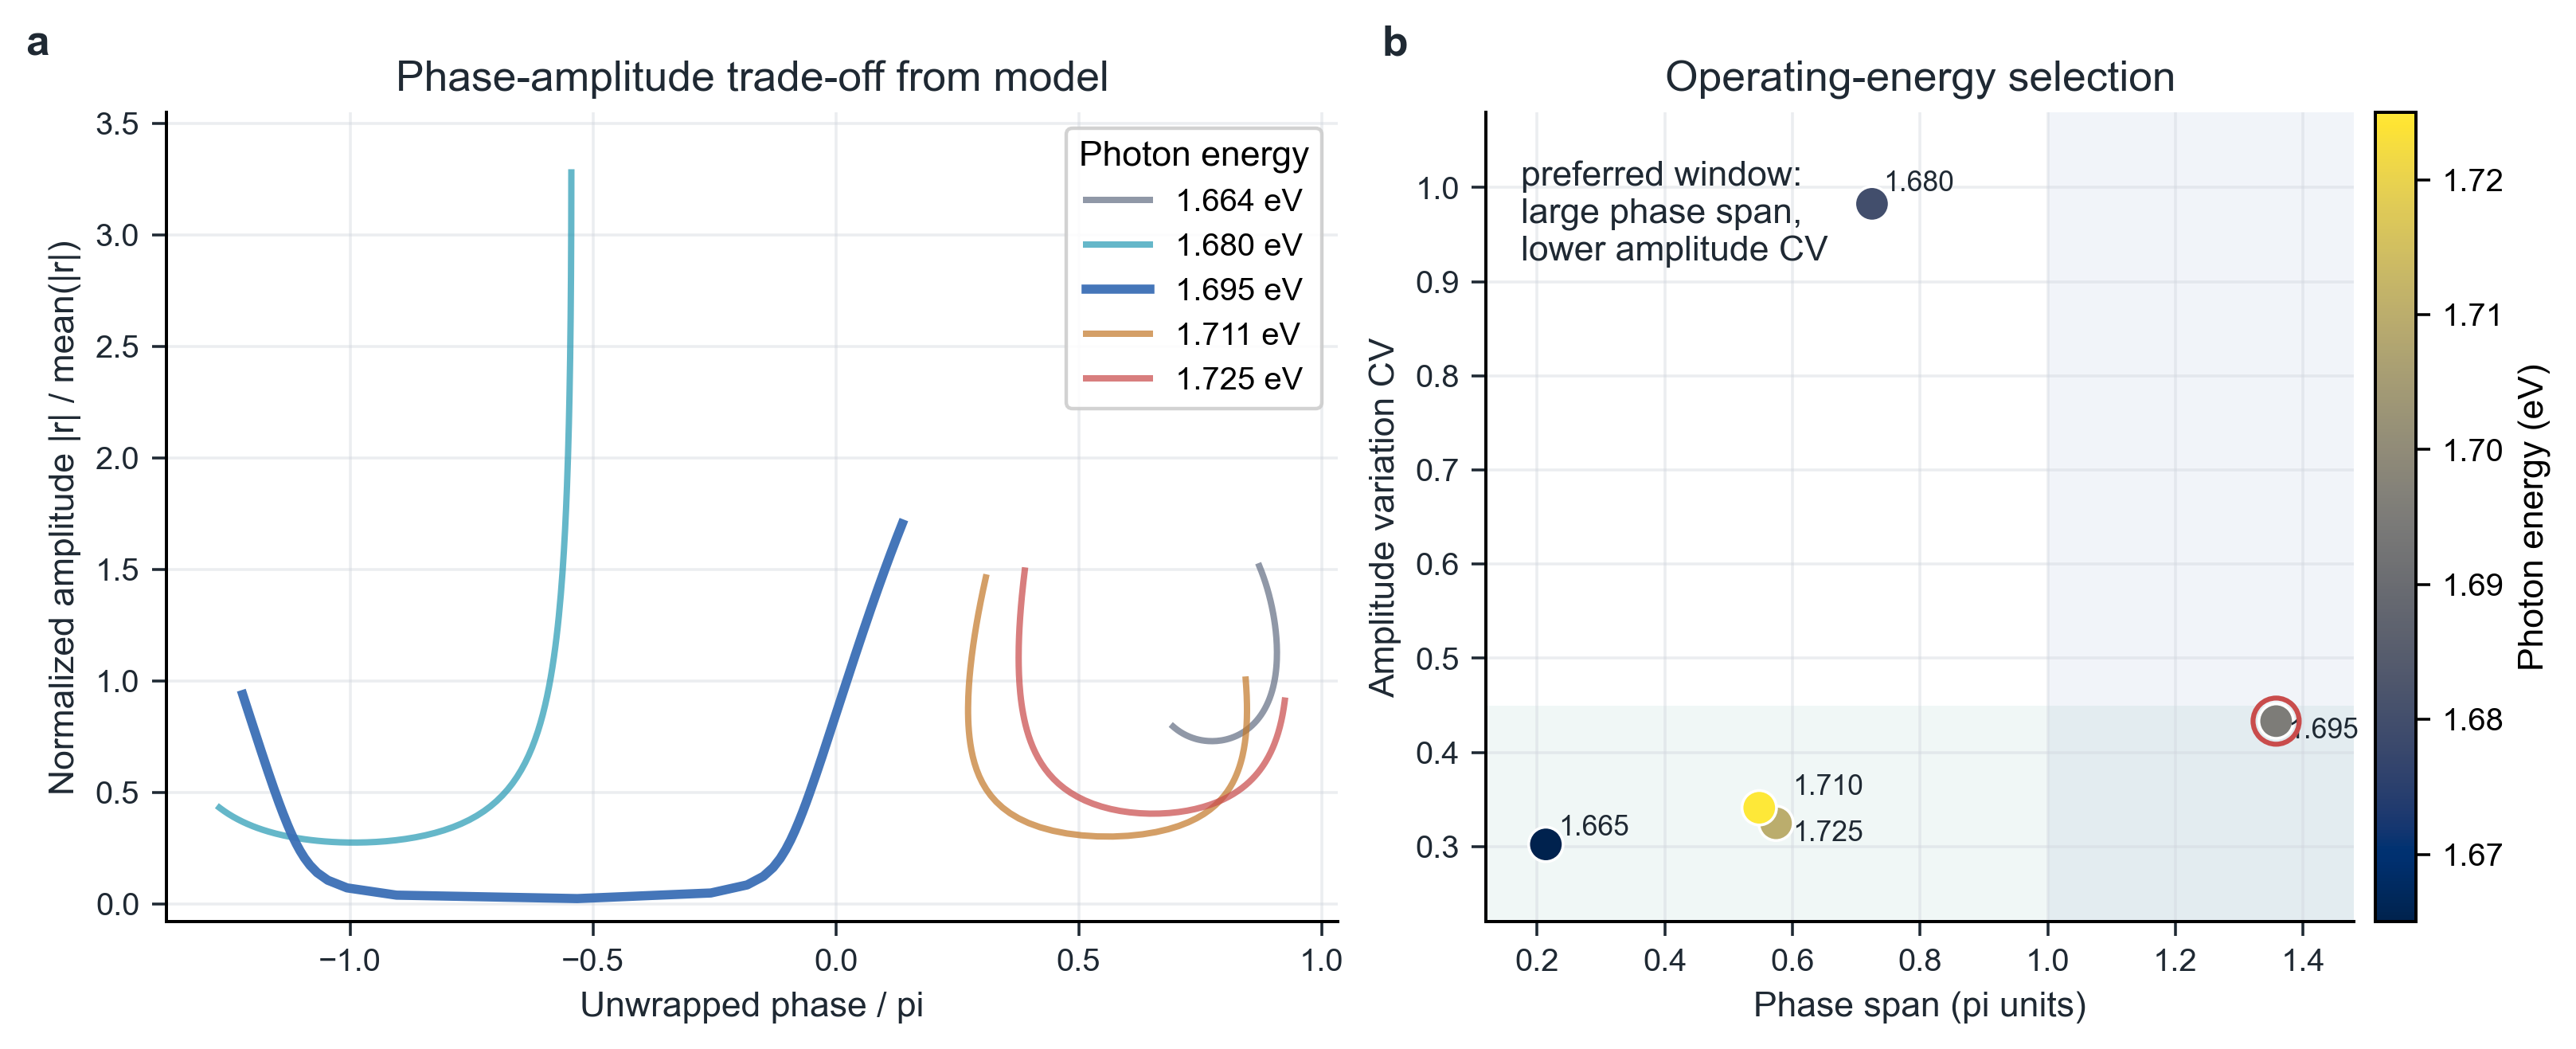
\includegraphics[width=\linewidth]{figure_5_amplitude_compensation.png}
  \caption{Phase--amplitude trade-off from the coupled-oscillator model。不同 photon energy 工作点给出不同的 phase span 与 normalized amplitude fluctuation（CV）。该图用于选择 design energy，替代原先手工 one-layer/two-layer amplitude-compensation 曲线。}
  \label{fig:amplitude-compensation}
\end{figure}

\section{实验验证判据}

实验验证不是只看一张谱图，而是检查设计闭环是否成立：
\begin{itemize}
  \item 在 $R(E,\vg)$ 中观察 gate-tuned strong-to-weak coupling transition；
  \item 在 design energy 下提取可用的 $|r(\vg)|$ 与 $\phi(\vg)$ 控制窗口；
  \item 对目标角反推出可施加的 gate voltage map；
  \item 在 Fourier plane 中验证 reflected far-field peak 是否移动到设定角；
  \item 比较不同工作能量下 phase span 与 amplitude CV 的取舍。
\end{itemize}

当前 Python 结果给出明确的预测：$0^\circ$、$10^\circ$、$20^\circ$ 三个目标角对应的主瓣位置与设计角一致，同时 Figure 5 给出工作能量选择时 phase span 与 amplitude CV 的取舍。这说明该 proposal 在模型层面具备自洽的设计--预测--控制--验证链条。

\section{边界与结论}

需要强调的是，本报告中的图来自 deterministic Python design simulation。它们不是 measured spectra，不是 COMSOL/FDTD full-wave calculation，也不代表实验已经完成。文献中的 9.9 dB reflectance modulation 是 B1 optical modulation device 的实验结果，不能直接写成本项目 beam-steering device 的已实现结果。

项目同时导出了 Origin 版本图件和 CSV 源数据，便于后续在 Origin 中继续排版；这些 Origin 图使用同一套 deterministic model data，不构成独立实验或 full-wave 仿真证据。

本项目的价值在于提出了一个可解释、可测试、可用 Python 预验证的创新实验方案：以 active vdW excitonic beam steering 为平台，以 electrically tunable strong coupling 为新机制，把 bare-exciton phased array 推进到 gate-tunable exciton-polariton phased array。若实验中能够完成 $R(E,\vg)$ 测量、complex reflection extraction、voltage-map programming 和 Fourier-plane verification，就可以系统检验电控强耦合在 programmable beam steering 中的作用。

\begin{thebibliography}{9}

\bibitem{li2023}
Melissa Li, Claudio U. Hail, Souvik Biswas, and Harry A. Atwater.
\newblock Excitonic Beam Steering in an Active van der Waals Metasurface.
\newblock \emph{Nano Letters}, 23(7), 2023.
\newblock DOI: \href{https://doi.org/10.1021/acs.nanolett.3c00032}{10.1021/acs.nanolett.3c00032}.

\bibitem{hoekstra2026strong}
Tom Hoekstra and Jorik van de Groep.
\newblock Electrically tunable strong coupling in a hybrid-2D excitonic metasurface for optical modulation.
\newblock \emph{Light: Science \& Applications}, 15, 28, 2026.
\newblock DOI: \href{https://doi.org/10.1038/s41377-025-02079-3}{10.1038/s41377-025-02079-3}.

\bibitem{hoekstra2026complex}
Tom Hoekstra, Mark L. Brongersma, and Jorik van de Groep.
\newblock Hybrid-2D Excitonic Metasurfaces for Complex Amplitude Modulation.
\newblock \emph{Nano Letters}, 26(18), 2026.
\newblock DOI: \href{https://doi.org/10.1021/acs.nanolett.6c00072}{10.1021/acs.nanolett.6c00072}.

\end{thebibliography}

\end{document}
